\documentclass{article}
\usepackage{graphicx} % Required for inserting images
\usepackage{geometry}
\usepackage{biblatex}
\addbibresource{bib.bib}
\geometry{letterpaper, margin=1in}

\usepackage{float} % table captions on top
\floatstyle{plaintop}
\restylefloat{table}

\begin{document}

\begin{center}
\bfseries Computing at Scale

Midterm Progress - Mikiel Gica
\end{center}

Work throughout the first half of the semester involved the development of an anisotropic size field that results
in anisotropic elements on the shock when used by a mesh adapter. The anisotropic size field is evaluated at mesh
vertices, and the normal size depends on the distance of the vertex from the shock. For our purposes, the shock is not
part of the mesh being adapted, so mesh vertices may not necessarily lie on the shock surface. If a mesh vertex is 
sufficiently far from the shock, the mesh adapter may evaluate the size of the vertex to be too large, and fail to
place anisotropic elements on the shock. An analytic anisotropic size field was formulated that works reasonably well
with SCOREC MDS adapt, and could work well on Simmetrix's mesh adapter, given enough adapt iterations.

The size field was tested on a double cone geometry split in half with "manufactured" shock data (made up shock geometry for testing). 
To increase performance, the size field is based on a shock distance determined with analytic equations. Initial meshes were generated with meshing software Simmetrix SimModeler and Capstone. 
The initial mesh was adapted with both SCOREC MDS adapt and Simmetrix adapt using an analytic anisotropic size field. Figure \ref{fig:result} is an example of an adapted mesh.

\begin{figure}[H]
\centering
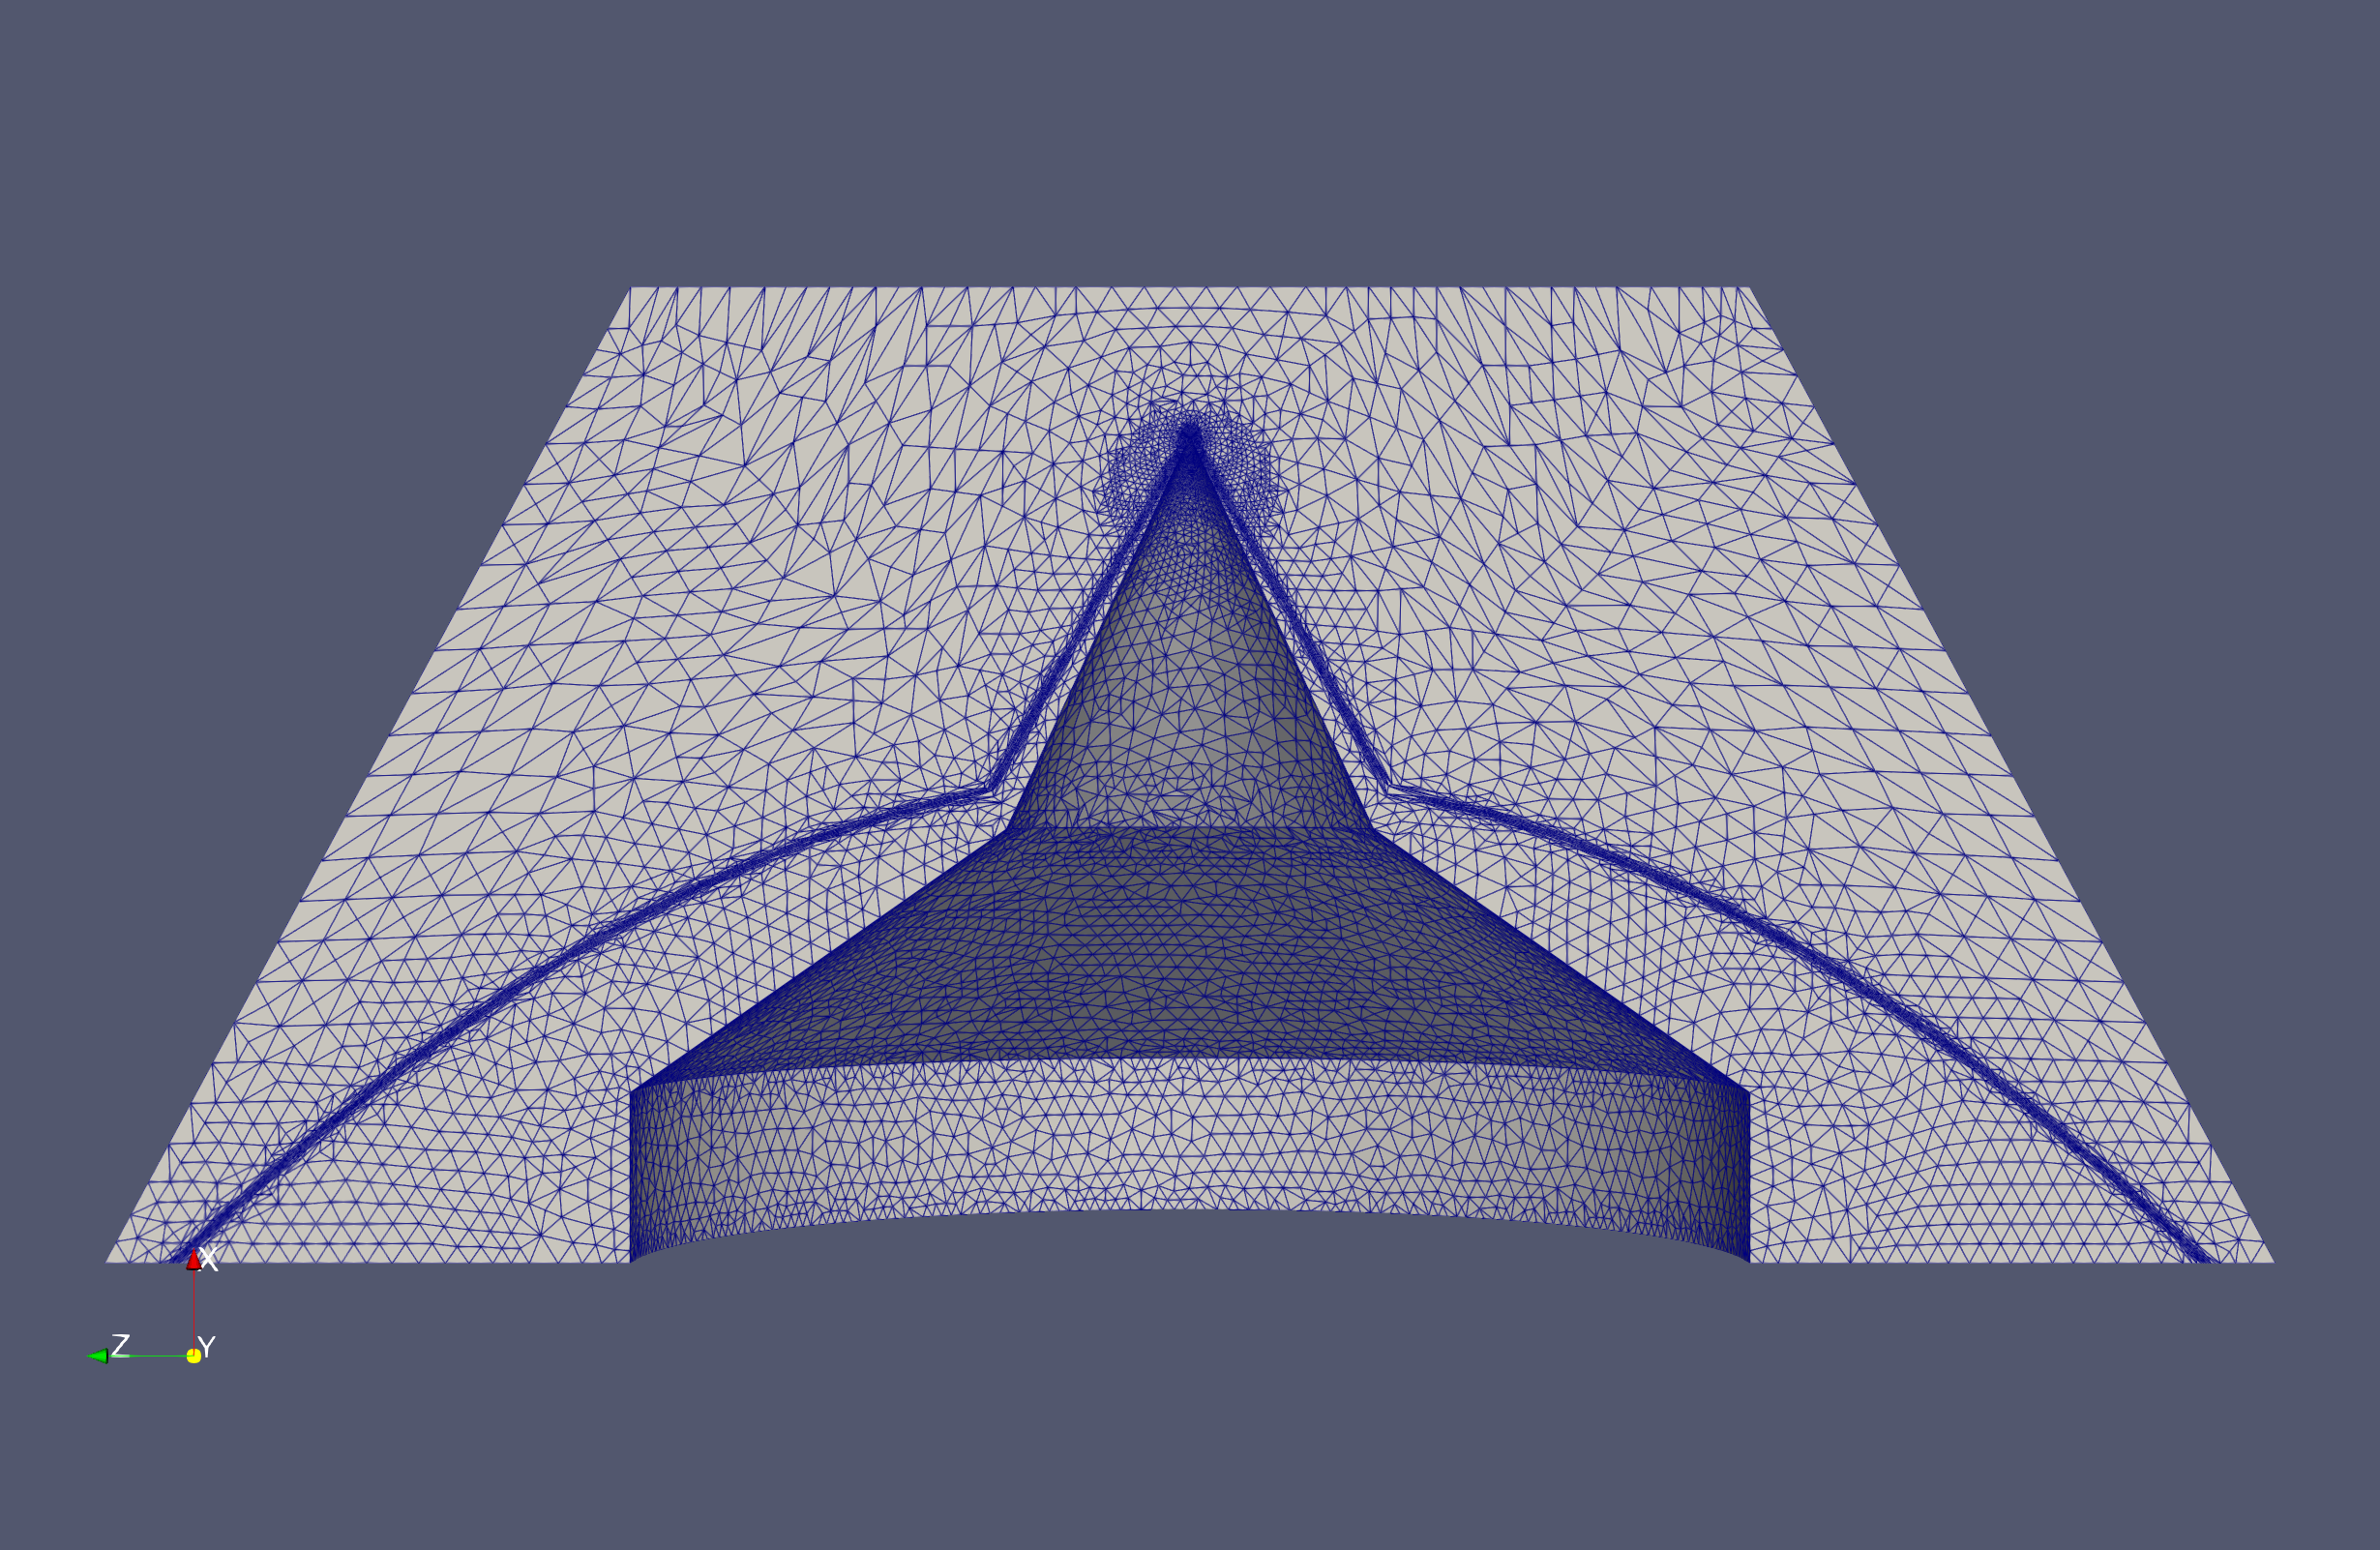
\includegraphics[width=6in]{after_AF_wholeview.png}
\caption{Example adaptation result using SCOREC MDS adapt}
\label{fig:result}
\end{figure}


The next steps would be to generalize the anisotropic size field formulated for the double cone case for use in other
problems and implement this in the Adaptation Controller software. The anisotropic size field implementation will have the
appropriate automated tests in place. The automated tests for the size field will involve cases with manufactured shock data
such as the double cone case. After the implementation of an appropriate anisotropic size field in the Adaptation Controller, the usage of real shock data
will be attempted and tested accordingly.

\end{document}